
队列是一个非常简单的数据结构,可以从两端访问的数组:数据添加到数组的队尾,在队头删除数据。实现时,队列和堆栈还是有一些区别和相似的,接下来我们会经常将队列和堆栈进行对比。

就像堆栈一样,STL也有队列容器\texttt{std::queue},当涉及到并发性时,也有相同的问题:删除元素的接口不是事务性的,需要三个独立的成员函数共同完成。如果使用带有锁的\texttt{std::queue}创建一个线程安全的队列,就必须像堆栈那样对其进行包装:

\hspace*{\fill} \\ %插入空行
\noindent
\textbf{03\_queue.C}
\begin{lstlisting}[style=styleCXX]
template <typename T> class mt_queue {
	std::queue<T> s_;
	mutable spinlock l_;
	public:
	void push(const T& v) {
		std::lock_guard g(l_);
		s_.push(v);
	}
	std::optional<T> pop() {
		std::lock_guard g(l_);
		if (s_.empty()) {
			return std::optional<T>(std::nullopt);
		} else {
			std::optional<T> res(std::move(s_.front()));
			s_.pop();
			return res;
		}
	}
};
\end{lstlisting}

这里使用自旋锁(比互斥锁快)。\texttt{front()}的实现方式与\texttt{pop()}相似,只是不需要删除头部元素。基准测试会测量“一个元素推入队列,并将其弹出”所花费的时间。使用上一节中做测试的x86机器,可以得到以下的结果:

%\hspace*{\fill} \\ %插入空行
\begin{center}
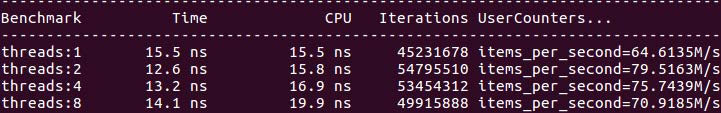
\includegraphics[width=0.9\textwidth]{content/2/chapter7/images/17.jpg}\\
图7.17 - 由自旋锁保护的\texttt{std::queue}性能
\end{center}

为了进行比较,在相同的硬件上,没有锁的\texttt{std::queue}每秒可以发送280M个元素(一个item表示\texttt{push}和\texttt{pop},所以这里测试的是每秒可以通过队列吞吐多少个元素)。其结果与堆栈的情况非常相似,为了比锁保护的版本更好,必须尝试一下无锁实现。

\subsubsubsection{7.4.1\hspace{0.2cm}无锁队列}

开始设计无锁队列之前,要对每个事务进行详细的分析,就像对堆栈那样。同样,假设队列建立在一个数组或类似数组的容器上(这里推迟讨论关于数组存满时会发生的问题)。将元素推入队列看起来就像堆栈一样:

%\hspace*{\fill} \\ %插入空行
\begin{center}
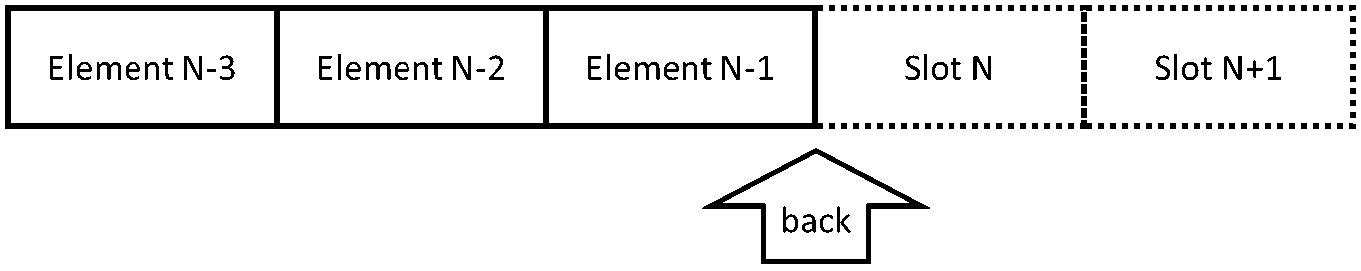
\includegraphics[width=0.9\textwidth]{content/2/chapter7/images/18.jpg}\\
图7.18 - 在队列尾部添加元素(生产者视角)
\end{center}

这里需要数组中第一个空槽的下标。然而,从队列中删除元素与在堆栈上的相同操作不同。可以在图7.19中看到(与图7.9比较):

%\hspace*{\fill} \\ %插入空行
\begin{center}
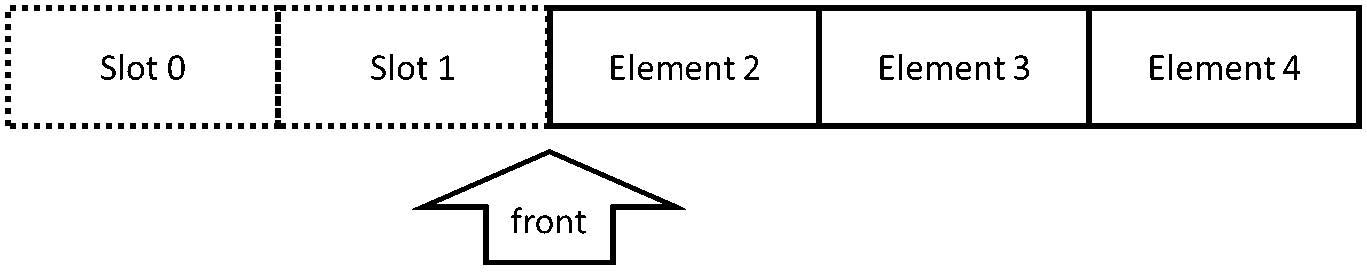
\includegraphics[width=0.9\textwidth]{content/2/chapter7/images/19.jpg}\\
图7.19 - 在队头部移除元素(消费者视角)
\end{center}

元素从队列的头部删除,因此需要尚未删除的第一个元素的索引(队列当前的头)。

现在来看看队列和堆栈之间的区别。堆栈中,生产者和消费者都在同一个位置上操作:堆栈的顶部。若生产者开始在堆栈顶部构造新元素,消费者就必须等待其完成。\texttt{pop}操作不能返回最后一个构造的元素,而不会在数组中留下一个空洞,而且在构造完成之前,不能返回正在构造的元素。

对于队列来说,情况就不同了。只要队列不是空的,生产者和消费者就根本不会交互。\texttt{push}操作不需要知道头部的索引是什么,而\texttt{pop}操作不关心队尾的索引。生产者和消费者不会对同一内存位置的访问进行竞争。

当遇到这样的情况,即有几种不同的方式来访问数据结构,并且它们(大多数)不相互交互。建议首先考虑将这些角色分配给不同线程的场景,进一步简化使用每一种线程的方式。我们的例子中,其意味着一个生产者线程和一个消费者线程。 

因为只有生产者需要访问返回索引,而且只有一个生产者线程,不需要为这个索引使用原子整数。类似地,索引只是普通整数。在队列变为空时,两个线程才会交互。为此,需要一个原子变量,表示队列的大小。生产者在第一个空槽中构造新元素,并向前推进返回索引(可以以任何顺序,因为只有一个生产者线程)。然后,增加队列的大小,以反映队列现有的元素数量。 

消费者必须按相反的顺序操作。检查队列大小,确保队列不为空。然后消费者可以从队列中获取第一个元素,并推进队列头部的索引。当然,不能保证在检查和访问头部元素时,队列大小不会改变。但这也不会引起任何问题。因为,只有一个消费者线程,而生产者线程只能增加队列大小。

在探索堆栈的过程中,没讨论向数组添加更多内存的问题,并假设已知堆栈的最大容量,并且不会超过(如果超过了该容量,也可以使\texttt{push}操作失败)。对于队列来说,同样的假设就不够了。随着元素的添加和从队列中删除,前后的索引都会移动,并最终到达数组的末尾。当然,数组的第一个元素未使用,所以最简单的解决方案是将数组视为循环缓冲区,并对数组下标使用取模运算:

\hspace*{\fill} \\ %插入空行
\noindent
\textbf{03a\_atomic\_pc\_queue.C}
\begin{lstlisting}[style=styleCXX]
template <typename T> class pc_queue {
public:
	explicit pc_queue(size_t capacity) : 
	capacity_(capacity),
	data_(static_cast<T*>(::malloc(sizeof(T)*capacity_))) {}
	~pc_queue() { ::free(data_); }
	bool push(const T& v) {
		if (size_.load(std::memory_order_relaxed) >= capacity_)
		return false;
		new (data_ + (back_ % capacity_)) T(v);
		++back_;
		size_.fetch_add(1, std::memory_order_release);
		return true;
	}
	std::optional<T> pop() {
		if (size_.load(std::memory_order_acquire) == 0) {
			return std::optional<T>(std::nullopt);
		} else {
			std::optional<T> res(
			std::move(data_[front_ % capacity_]));
			data_[front_ % capacity_].~T();
			++front_;
			size_.fetch_sub(1, std::memory_order_relaxed);
			return res;
		}
	}
private:
	const size_t capacity_;
	T* const data_;
	size_t front_ = 0;
	size_t back_ = 0;
	std::atomic<size_t> size_;
};
\end{lstlisting}

队列需要一个特殊的基准测试,因为在设计上受了一些限制:一个生产者线程和一个消费者线程:

\hspace*{\fill} \\ %插入空行
\noindent
\textbf{03a\_atomic\_pc\_queue.C}
\begin{lstlisting}[style=styleCXX]
pc_queue<size_t> q(1UL<<20);
void BM_queue_prod_cons(benchmark::State& state) {
	const bool producer = state.thread_index & 1;
	const size_t N = state.range(0);
	for (auto _ : state) {
		if (producer) {
			for (size_t i = 0; i < N; ++i) q.push(i);
		} else {
			for (size_t i = 0; i < N; ++i) 
			benchmark::DoNotOptimize(q.pop());
		}
	}
	state.SetItemsProcessed(state.iterations()*N);
}
BENCHMARK(BM_queue_prod_cons)->Arg(1)->Threads(2)
->UseRealTime();
BENCHMARK_MAIN();
\end{lstlisting}

为了进行比较,应该在相同的条件下对锁保护的队列进行基准测试(锁的性能通常对线程竞争非常敏感)。同一台x86机器上,两个队列的吞吐量大致相同,为每秒100M个整数元素。在ARM处理器上,锁相对来说更耗时,我们的队列也不例外:

%\hspace*{\fill} \\ %插入空行
\begin{center}
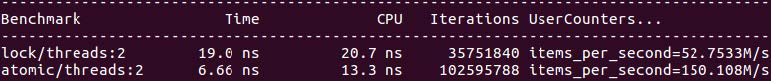
\includegraphics[width=0.9\textwidth]{content/2/chapter7/images/20.jpg}\\
图7.20 - ARM上基于锁的整数队列与无锁整数队列的性能对比
\end{center}

即使是在x86上,分析也不完整。前一节中,若堆栈元素很大,那么复制所需的时间要长于线程同步(锁定或原子操作)。因为大多数时候,一个线程仍然需要等待另一个线程完成复制,所以不能充分利用使用这个堆栈,从而提出了替代方案:指针堆栈,将实际数据存储在其他地方。缺点是需要另一个线程安全的容器,来存储这些数据(程序需要将其存储在某个地方)。对于队列来说,这仍然是可行的建议,但现在有了另一个选择。队列中的生产者和消费者线程不会互相等待,它们的交互在检查大小后结束。如果数据元素很大,那么无锁队列就有优势,因为两个线程可以同时复制数据,并且比起线程竞争的时间要短得多。要进行这样的基准测试,只需要创建一个大型对象队列,比如一个包含大型数组的结构体。即使是在x86硬件上,也如预期的一样,无锁队列执行的更快:

%\hspace*{\fill} \\ %插入空行
\begin{center}
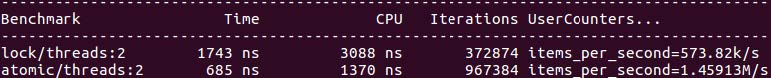
\includegraphics[width=0.9\textwidth]{content/2/chapter7/images/21.jpg}\\
图7.21 - x86上基于锁的队列与无锁队列的性能对比
\end{center}

即使有强加的限制,这也是非常有用的数据结构。当已知队列元素数量的上限时,这个队列可以用于在生产者和消费者线程之间传输数据,或者处理生产者在推送数据前的情况(等待)。队列非常高效,更重要的是它具有非常低的、可预测的延迟:队列本身没有锁,也没有等待。线程间不需要互相等待,除非队列已满。如果消费者必须对队列中获取的数据元素进行处理,并且开始的消费能力小于队列增加的速度,这样队列很快会填满。这时,常见的方法是让生产者处理不能入队的元素。这将在生产者线程产生延迟,直到消费者能够赶上生产的速率(因为会无序地处理数据,这种方法并不适用于每个程序,但通常非常高效)。

对于许多生产者或消费者线程的情况,队列的泛化将使实现更加复杂。即使使前后端索引原子化,基于原子的无等待算法也无法工作。如果多个消费者线程读取一个非零的值,这不再足以让其他线程继续。对于多个使用者,当一个线程检查发现非零时,大小可以减少,并变为零(在第一个线程测试大小之后,在尝试访问队列前端之前,其他线程弹出了所有元素)。

通用的解决方案是使用与堆栈相同的技术,将\texttt{front}和\texttt{back}索引打包到一个64位原子类型中,并使用比较-交换以原子方式访问。其实现类似于堆栈的实现,理解了上一节中的代码的读者可以来实现这个队列了。在文献中还可以找到其他无锁队列解决方案,本章将提供足够的背景知识来理解、比较和测试这些实现。

正确地实现复杂的无锁数据结构是很耗时的工作,需要技能和注意力。完成实现之前需要进行一些性能评估,这样就可以知道努力是否可能得到回报。这里使用模拟基准测试,将非线程安全数据结构(每个线程的本地)上的操作与共享变量(锁或原子数据)上的操作结合在一起。其目标是提出等效计算的代码,可以进行基准测试。不过,这样并不完美,如果有一个无锁队列的想法,有三个原子变量,每个原子变量上都有比较和交换操作,并且发现评估的基准测试要比自旋锁保护的队列慢好几倍,那么实现出来的队列就不太可能有好的回报。

对部分实现的代码进行基准测试的第二种方法是构造基准测试,以避免未实现的某些极端情况。如果希望队列在大部分时间内不为空,并且初始实现不处理空队列的情况,就应该对该实现进行基准测试,并限制基准测试,以便队列永远不会为空。这个基准测试将表明我们是否在正确的轨道上,将显示在非空队列情况下期望的性能。实际上,当堆栈或队列耗尽内存时,我们已经采用了这种方法。这里,只是简单地假设这种情况不会经常发生,并构建了基准测试来避免这种情况。

还有另一种类型的并发数据结构实现,使用起来很高效。接下要来了解一下。

\subsubsubsection{7.4.2\hspace{0.2cm}顺序不一致的数据结构}

首先回到最开始的问题,什么是队列?当然,是一种数据结构,首先添加的元素先检索。实现中,元素添加到底层数组的顺序保证了这一点。比如:新元素添加到前面,而旧元素从后面读取。

仔细检查一下这个定义是否仍然适用于并发队列。当从队列中读取一个元素时,执行如下代码:

\begin{lstlisting}[style=styleCXX]
T pop() {
	T return_value;
	return_value = data[back];
	--back;
	return return_value;
}
\end{lstlisting}

返回值可以包装在\texttt{std::optional}中或通过引用传递。关键是从队列中读取值,减少返回索引,并将元素值返回给调用者。多线程程序中,线程可以进行抢占。如果有两个线程A和B,并且线程A从队列中读取最旧的元素,有可能是线程B首先完成\texttt{pop()},并将其值返回给调用者。因此,如果按顺序将两个元素X和Y放入队列,并且有多个线程将它们取出并打印,那么程序将打印Y,然后打印X。当多个线程将元素推入队列时,会发生同样的重新排序。最终,即使队列保持严格的顺序(如果暂停程序并检查内存中的数组,元素顺序正确),程序其余部分退出队列的元素的顺序不能保证与进入队列的顺序一致。

当然,顺序也不是完全随机的。即使在并发程序中,堆栈看起来也与队列不同。从队列中检索到的数据的顺序与添加值的顺序大致相同,大规模重排很少发生(由于某种原因,当一个线程延迟了很长时间时,就会发生大规模重排)。

队列仍然会保留的属性是\textit{顺序一致性}。顺序一致产生的输出与所有线程一次执行一个操作(没有任何并发性)的程序的输出相同,任何特定线程执行操作的顺序都不会改变。换句话说,程序接受所有线程执行的操作序列,并可以交叉执行,但不会重新排序。

顺序一致性是一种便捷的属性,分析这类程序的行为要容易得多。在队列的情况下,线程A将两个元素X和Y入队,X先入队,然后是Y,并且线程B会将它们弹出队列,并且将以正确的顺序出现。另一方面,这两个元素可能由两个不同的线程弹出队列。这样,它们可以以任意顺序出现,所以程序必须能够处理这样的情况。

如果放弃顺序一致性,就为设计并发数据结构开辟了一种全新的方法。我们以队列来探讨,其基本思想是:可以有几个单线程子队列,而非单个线程安全队列。每个线程必须以原子的方式获得这些子队列中的所有权。最简单的实现方法是,使用指向子队列的原子指针数组,如图7.22所示。为了获得该队列的所有权,同时防止其他线程访问该队列,需要将子队列指针自动交换为空。

%\hspace*{\fill} \\ %插入空行
\begin{center}
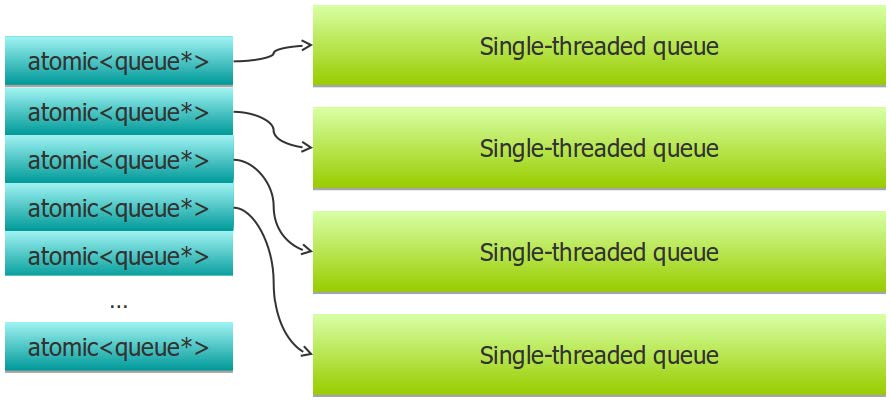
\includegraphics[width=0.7\textwidth]{content/2/chapter7/images/22.jpg}\\
图7.22 - 基于通过原子指针访问数组子队列的非顺序一致队列
\end{center}

需要访问队列的线程必须获得一个子队列,可以从指针数组的任何元素开始。如果为空,则该子队列当前处于繁忙状态,然后尝试下一个元素,以此类推,直到只剩下一个子队列。此时,只有一个线程在子队列上操作,因此不需要线程安全(子队列甚至可以是\texttt{std::queue})。操作(\texttt{push}或\texttt{pop})完成后,线程原子性地将子队列指针写回数组,将子队列的所有权返回给队列。

\texttt{push}操作必须继续尝试剩下的子队列,直到找到子队列为止(或者,可以允许\texttt{push}在尝试一定次数后失败,向调用者发出队列太忙的信号)。\texttt{pop}操作可能会保留一个子队列,结果发现是空的。这种情况下,必须尝试从另一个子队列中弹出(可以在队列中保持元素的原子计数,若队列是空的,可以快速返回)。

当然,\texttt{pop}可能在一个线程上失败,并报告队列为空。实际上,这并不是因为另一个线程将新数据推入队列。但这可能发生在并发队列上,一个线程检查队列大小,发现队列是空的,但在控制权返回给调用者之前,队列可能会成为非空队列。同样,顺序一致性对多个线程的可见性不一致性,需要进行了一些限制,而非顺序一致性队列使弹出元素的顺序变得不确定。尽管顺序有些乱,但还能接受。

不过,这并不是适用于所有数据结构,当大多数类似于队列顺序可以接受时,顺序不一致可以产生明显的性能提升,特别是在有许多线程的系统中。在一个运行许多线程的大型x86服务器上,进行顺序不一致队列扩展后的情况:

%\hspace*{\fill} \\ %插入空行
\noindent
\textbf{03b\_noncst\_queue.C}
\begin{center}
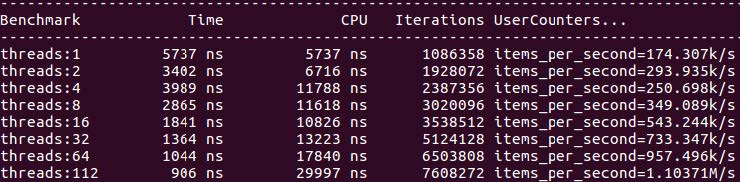
\includegraphics[width=0.9\textwidth]{content/2/chapter7/images/23.jpg}\\
图7.23 - 顺序不一致队列的性能
\end{center}

这个基准测试中,所有线程都执行\texttt{push}和\texttt{pop}操作,并且元素相当大(复制每个元素需要复制1KB的数据)。为了进行比较,自旋锁保护的\texttt{std::queue}在单个线程上具有相同的性能(大约每秒170k个元素),但根本没有扩展性(整个操作都是锁定的),而且性能下降得很慢(由于锁定的开销),对于最大线程数来说,性能会下降到(大约)每秒130k个元素。

当然,若出于性能考虑,可以接受顺序不一致程序的混乱,那么许多其他数据结构也可以使用这种方法。

当涉及到并发顺序容器(如堆栈和队列)时,我们要讨论的最后一个主题是如何处理需要更多内存的情况

\subsubsubsection{7.4.3\hspace{0.2cm}并行数据结构的内存管理}

现在来讨论内存管理的问题,之前假设数据结构的初始内存分配已经足够,至少对于不会使整个操作变成单线程的无锁数据结构来说是这样的。本章中看到锁保护的和顺序不一致的数据结构没有这个问题,在锁或抢占所有权的方式下,只有一个线程操作特定的数据结构,所以内存按照常规的方式分配。

对于无锁数据结构,内存分配是一个重大挑战。这通常是一个耗时的操作,特别是当数据必须复制到新位置时。多个线程可能会让数据结构的内存耗尽,通常只有一个线程可以添加新的内存(很难让那部分也变成多线程),其余的线程必须等待。对于这个问题没有较好的通用解决方案,这里只是给出一些建议。

首先,最好的选择是避免这个问题。当需要无锁数据结构时,可以估计其最大容量并预分配内存,例如:知道要进入队列的数据元素的总数。或者可以将问题推给调用者,可以告诉调用者数据结构的容量不足,而不是增加内存。对于无锁数据结构的性能来说,这可能是一个可以接受的折衷方案。

如果需要增加内存,最理想的做法是添加内存时,但不复制现有数据结构。这意味着不能简单地分配更多内存,并将所有内容复制到新位置。相反,必须将数据存储在固定大小的内存块中,就像\texttt{std::deque}一样。当需要更多内存时,会分配另一个内存块,通常会有一些指针地址需要更改,但不会复制数据。

完成内存分配的所有情况下,这是很少发生的事件。如果不是这样,那么使用由锁或独占所有权保护的单线程的数据结构就好。这个罕见事件的性能不是关键,可以简单地锁定整个数据结构,并让一个线程执行内存分配和必要的更新。关键的是公共内存地址,也就是意味着不需要更多内存的地址,所以程序会运行的很快。

这个想法非常简单,不希望每次都在每个线程上获取内存锁,串行化整个程序。也不需要这样做,大多数时候,不会内存不足,也不需要这个锁。因此,需要检查原子标志。只有当内存分配正在进行,并且所有线程都必须等待时,才会设置该标志:

\begin{lstlisting}[style=styleCXX]
std::atomic<int> wait; // 1 if managing memory
if (wait == 1) {
	… wait for memory allocation to complete …
}
if ( … out of memory … ) {
	wait = 1;
	… allocate more memory …
	wait = 0;
}
… do the operation normally … 
\end{lstlisting}

这里的问题是,多个线程可能会在设置等待标志之前同时检测内存不足的情况。然后,尝试向数据结构中添加更多的内存,这通常会导致竞争(重新分配底层内存很少是线程安全的)。不过,有一种简单的解决方案,称为\textbf{双重检查锁},它同时使用互斥锁(或另一个锁)和原子标志。如果标志没有设置,那么一切正常,可以照常进行。如果设置标志,则必须获取锁,并再次检查该标志:

\begin{lstlisting}[style=styleCXX]
std::atomic<int> wait;  // 1 if managing memory
std::mutex lock;
while (wait == 1) {};  // Memory allocation in progress
if ( … out of memory … ) {
	std::lock_guard g(lock);
	if (… out of memory …) { // We got here first!
		wait = 1;
		… allocate more memory …
		wait = 0;
	}
}
… do the operation normally …
\end{lstlisting}

第一次,检查内存不足的情况,没有任何锁。速度很快,大多数时候,不会遇到内存不足。第二次,在锁下检查它,在锁下可以保证一次只有一个线程在执行。多线程可能会检测到内存不足,但第一个获得锁的线程是处理这种情况的线程,所有剩余的线程都在等待锁。当它们获得锁时,则进行第二次检查(因此,双重检查锁),发现内存充足。

这种方法可以泛化来处理罕见的特殊情况,但与其他代码相比,以无锁的方式实现这种情况要困难得多。某些情况下,甚至可能对空队列的情况非常有用。如果两个线程组不相互交互,那么多个生产者或多个消费者的处理将需要原子递增的索引。如果在特定的应用程序中,就能够保证队列很少(如果有的话)变成空,那么可以选择对于非空队列来说非常快(无需等待)的实现,但如果队列可能为空,则需要使用全局锁。

好了,我们已经详细地介绍了顺序数据结构,接下来来研究一下节点数据结构。






























